\documentclass[runningheads]{class}
% Packages
\usepackage[
	a4paper,
	left=44mm,
	right=44mm,
	top=52mm,
	bottom=52mm
]{geometry}
\usepackage[polish]{babel}
\usepackage[utf8]{inputenc}
\usepackage[T1]{fontenc}
\usepackage[
	colorlinks=true,
	citecolor=black,
	linkcolor=black,
	urlcolor=blue,
	bookmarksopen=true
]{hyperref} % hyperref is necessary for \emailsubj of used class
%\usepackage{bm} % bold math symbols
%\usepackage{tikz} % creating graphic vectors
%\usepackage{pgfplots} % plots
\usepackage{enumitem} % control over itemize, enumerate
\usepackage{array}
\usepackage{amsmath}
\usepackage{algorithm}
\usepackage{algpseudocode}

\usepackage{subfig}
\usepackage{hyperref}
\usepackage{graphicx}
\usepackage{caption}
\usepackage{float}
% Paths
% Geometry
\setlist{topsep=4pt}
% Caption font
% https://en.wikibooks.org/wiki/LaTeX/Fonts#Built-in_sizes
\captionsetup[figure]{font=small, labelfont=bf}
\captionsetup[table]{font=small, labelfont=bf}
% Commands
\renewcommand\UrlFont{\color{blue}\rmfamily} % blue roman url font, Springer's eBook style
\newcolumntype{A}{>{}m{2.2cm}}
\newcolumntype{B}{>{}m{9cm}}
\newcommand\dummyemail{
	\hypersetup{urlcolor=black}
	\emailsubj[gall.anonim.stud@pw.edu.pl]{Warning! Provided e-mail address is dummy. Do not send a message.}
}
\floatname{algorithm}{Listing} % name
\newcommand{\wek}[1]{
    {\bf #1} 
}
\newcommand{\mat}[1]{
    {\bf #1} 
}
\newcommand{\srednia}[1]{
    \langle #1 \rangle 
}
\newcommand{\argmax}{\operatornamewithlimits{argmax}} 
\newcommand{\FES}{
    \text {FES} 
}
\newcommand{\MAXFES}{
    \text{MAXFES} 
}
\newcommand*{\tran}{{\mkern-1.5mu\mathsf{T}}}


\title{Modyfikacja reguł adaptacji macierzy kowariancji oraz zasięgu mutacji w strategiach ewolucyjnych}
\titlerunning{Modyfikacja reguł adaptacji w strategiach ewolucyjnych}
\author{Eryk Warchulski}
\authorrunning{Eryk Warchulski}
\institute{Instytut Informatyki, Politechnika Warszawska\\
\email{eryk.warchulski.stud@pw.edu.pl}
}
\begin{document}
\maketitle
\begin{abstract}
  W niniejszym artykule podejmuję problem modyfikacji dotychczasowych reguł adaptacji macierzy kowariancji oraz zasięgu mutacji w metodach strategii ewolucyjnych.
  Proponuję trzy metody kontroli zasięgu mutacji. Każda z nich bazuje na wartości funkcji celu punktu środkowego oraz na uproszczonej regule adaptacji macierzy kowariancji.
  Na podstawie przeprowadzonych przeze mnie eksperymentów wynika, że osiągane przez nie wyniki na standaryzowanych problemach testowych zdefiniowanych w ramach konkursu \texttt{CEC'2017} sugerują konkurencyjność wobec obecnie stosowanych modyfikacji. 
	\keywords{
    Strategie ewolucyjne, optymalizacja, CMA-ES, CSA
	}
\end{abstract}
% Content
\section{Wprowadzenie}
\label{section:wprowadzenie}
Strategia ewolucyjna z adaptacją macierzy kowariancji (ang. Covariance Matrix Adaptation Evolution Strategy, CMA-ES) \cite{cmaes} znajduje się w czołówce metod optymalizacyjnych w ramach konkursów \texttt{IEEE CEC} \cite{cec2017} oraz \texttt{BBOB} \cite{HansenEtal10}. W każdej iteracji algorytm tworzy populację złożoną z punktów wylosowanych przy użyciu wielowymiarowego rozkładu normalnego, którego parametry, tj. wektor wartości oczekiwanej oraz macierz kowariancji, są modyfikowane. Modyfikacja tych parametrów odbywa sie na podstawie reguły CMA (ang. Covariance Matrix Adaptation). Wskutek działaniapowyższej reguły funkcja gęstości prawdopodobieństwa lokalnie aproksymuje funkcję celu i tym samym zwiększa szansę na wylosowanie punktów blisko optimum lokalnego. Dynamika adaptacji rozkładu normalnego sterowana jest również przez kontrolę zasięgu mutacji, która bazuje na mechanizmie ścieżki ewolucyjnej (ang. evolution path) \cite{Hansen2001}. Zwiększona efektywność działania algorytmu wkustek stosowania powyższych mechanizmów jest okupiona znaczącym narzutem obliczeniowym, który często ogranicza zakres praktycznych zastosowań metody.
W artykule tym proponuję modyfikację działania algorytmu \texttt{CMA-ES}, które pozwalają zredukować złożoność obliczeniową metody przy niewielkiej stracie efektywności działania. Proponowane przeze mnie modyfikacje dotyczą reguły adaptacji macierzy kowariancji oraz zasięgu mutacji. Zmiana sposobu sterowania zasięgiem mutacji bazuje na kontroli punktu środkowego populacji \cite{Arabas17}, a zmiany dotyczące adaptacji macierzy kowariancji na pomyśle roważanym przez Beyer'a \cite{SMAES}.
Artykuł ten posiada następującą strukturę. W sekcji (\ref{section:adaptacje}) krótko przedstawiam zasadę działania algorytmu \texttt{CMA-ES} oraz nakreślam problemy związane ze złożonością obliczeniową w jego kanonicznej wersji. Omawiam również dotychczasowe próby rozwiązania tego problemu. Dokładny opis proponowanych przeze mnie metod znajduje się w sekcji (\ref{section:modyfikacje}). Sekcja (\ref{section:eskperymenty}) zawiera komentarz do rezultatów osiągniętych w ramach eksperymentów numerycznych. Sekcja ostatnia, (\ref{section5:podsumowanie}), stanowi podsumowanie artykułu oraz omawiam w niej plan dalszych badań.

\section{Mechanizmy adaptacyjne}
Pseudokod zawarty na wypisie (\ref{alg-CMA-ES}) przedstawia kanoniczną wersję algorytmu \texttt{CMA-ES}. Metoda steruje trzema parametrami: wektorem oczekiwanym $\wek{m}^{t}$, macierzą kowariancji
$\mat{C}^t$ oraz zasięgiem mutacji $\sigma^t$. Parametry te specyfikują wielowymiarowy rozkład normalny, który służy do tworzenia nowych punktów. Indeks górny $t$ oznacza numer iteracji algorytmu.
W każdej iteracji algorytm przy pomocy rozkładu normalnego z zerową wartoścoią oczekiwaną oraz macierzą kowariancji $\mat{C}^t}$ generuje zbiór wektorów $\{\wek{d}_1^t,...,\wek{d}_\lambda^t\}$ (linia 6). 
Wektory te służą do zaburzenia obecnego w danej iteracji wektora wartości oczekiwanej $\wek{m}^t$ wskutek czego powstają wektory pochodne $\wek{x}^t_i=\wek{m}^t+\sigma^t \wek{d}_i^t$.
Zbiór wektorów pochodnych jest sortowany malejąco (linia 10). Ze zbioru $\lambda$ wektorów wydzielany jest podzbiór $\mu$ wektorów o najmniejszej wartości funkcji celu. Podzbiór ten służy do
aktualizacji parametrów algorytmu. \\
Wartość oczekiwana $\wek{m}^t$ rozkładu aktualizowana jest wskutek zsumowania jej ze średnią ważoną wyselekcjonowanych wektorów $\wek{d}_{i}^{t}$. Wagi $w_{i]$ powinny być liczbami dodatnimi, których suma wynosi $1$ \cite{HansenOstermeier01}.
\begin{algorithm}[h]
\caption{CMA-ES}
\label{alg-CMA-ES}
\begin{algorithmic}[1]
\STATE $t \gets 1$
\STATE initialize$(\wek{m}^1,\sigma^1, C^1)$
\STATE $\wek{p}_c^1 \gets \wek{0}$, $\wek{p}_\sigma^1 \gets \wek{0}$
\WHILE{!stop}
   \FOR{$i=1$ \TO $\lambda$}
      \STATE $ \wek{d}_i^t \sim N(\wek{0}, \mat{C}^t) $
      \STATE $\wek{x}_i^t=\wek{m}^{t} + \sigma^t \wek{d}_i^t $
      \STATE evaluate $(\wek{x}_i^t)$
   \ENDFOR
   \STATE sort $ \left(\{ \wek{x}_i^t \} \right) $
  
   \STATE $\wek{\Delta}^{t} \gets \sum_{i=1}^\mu w_i \wek{d}_i^t $
   \STATE $\wek{m}^{t+1} \gets \wek{m}^{t+1} + \sigma^t \wek{\Delta}^{t} $
   \STATE $\wek{p}_c^{t+1} \gets (1-c_p)\wek{p}_c^t + \sqrt{\mu_\text{eff} c_p(2-c_p)} \cdot \wek{\Delta}^{t}$ where \newline
          $\qquad \mu_\text{eff}=1/\left(\sum_{i=1}^\mu (w_i)^2\right)$
   \STATE $\mat{C}^{t+1} \gets (1-c_1-c_\mu)\mat{C}^t + c_1 \mat{C}^t_1 + c_\mu  \mat{C}^t_\mu$ where \newline
$\qquad \mat{C}_\mu^t=\frac{1}{\mu_\text{eff}}\sum_{i=1}^\mu w_i(\wek{d}_i^t)(\wek{d}_i^t)^\tran$, \newline
$\qquad \mat{C}_1^t=(\wek{p}_c^t)(\wek{p}_c^t)^\tran$

   \STATE $\sigma^{t+1} \gets $ CSA $(\sigma^t, \mat{C}^{t}, \wek{\Delta}^{t})$ 
      
   \STATE $t \gets t+1$
\ENDWHILE
\end{algorithmic}
\end{algorithm}
Sposób aktualizacji macierzy kowariancji oraz parametru zasięgu mutacji ze względu na jego znaczenie opisałem kolejno w sekcji (\ref{CMA}) oraz (\ref{CSA}).
\subsection{Adaptacja macierzy kowariancji \label{CMA}}
  Macierz kowariancji $\mat{C}^{t+1}}$ wyliczana jest jako suma złożona z dwóch składników. Pierwszy z nich, $\mat{C}^t_\mu$, jest macierzą rangi $\mu$, która powstaje jako ważona suma iloczynu zewnętrznego $\mu$ wektorów  $\wek{d}_{i}^{t}$. Drugi z nich,  $\mat{C}^t_1$, jest macierzą o rzędzie równym 1 powstałą jako iloczyn zewnętrzny wektora $\wek{p}_c^t$. Wektor ten jest jedną ze ścieżek ewolucyjnych, które utrzymuje algortym w ramach swojego działania. 
  Oba składniki mają na celu zwiększenie prawdopodobieństwa wylosowania wektorów w kierunku poprawy, tj. mniejszej wartości funkcji celu. Wkład macierzy $\mat{C}^t_\mu$ reprezentuje zysk, który przynosi selekcja osobników, a z kolei macierz $\mat{C}^t_1$ -- zysk wnoszony przez ścieżkę ewolucyjną $\wek{p}_c^t$. Ścieżkę tę należy rozumieć jako trajektorię populacji zgodnie z którą kierunki tworzenia nowych punktów były najlepsze \cite{evol-path}.
\subsection{Kumulatywna adaptacja zasięgu mutacji \label{CSA}}
Sposób aktualizowania zasięgu mutacji $\sigma^t$ oparty jest na poniższym rozumowaniu. Niech funkcja celu $f$ będzie funkcją stałą. Wówczas składowe wektorów $\wek{d}_i^t$ nie posiadają korelacji z ich położeniem w przestrzeni.
Konsekwencją tego jest fakt, że wyselekcjonowane wektory  $\wek{d}_i^t$ są niezależne oraz zgodne z rozkładem $\mathcal{N}(0, \mat{C}^{t})$. W wyniku przekształcenia
  \begin{equation}
    (\mat{C}^{t})^{-\frac{1}{2}}\wek{d}_{i}^{t}
  \end{equation}
  wektory będą zgodne z izotropowym rozkładem normalnym, tj. $\mathcal{N}(0, I)$. W związku z powżyszym wektor $(\mat{C}^t)^{-1/2} \wek{\Delta}^t$ będzie posiadał rozkład normalny z zerową wartością oczekiwaną
  oraz macierzą kowariancji równą:
  \begin{equation}
    \Sigma((\mat{C}^t)^{-1/2} \wek{\Delta}^t) = \sum_{i=1}^\mu (w_i)^2 \mat{I}=\frac{1}{\mu_\text{eff}} \mat{I}
    \label{eq:01}
  \end{equation}

\floatname{algorithm}{Procedure}
\setcounter{algorithm}{0}
\begin{algorithm}[h]
\caption{CSA}
\begin{algorithmic}[1]
   \STATE $\wek{p}_\sigma^{t+1} \gets (1-c_s)\wek{p}_\sigma^t + \sqrt{\mu_\text{eff} c_s(2-c_s)} \cdot (\mat{C}^t)^{-\frac{1}{2}}\wek{\Delta}^t$
   \STATE $\sigma^{t+1} \gets \sigma^t \exp\left(\frac{c_s}{d_\sigma} \left(\frac{\| \wek{p}_\sigma^{t+1} \|}{E\|N(\wek{0},\mat{I})\|}-1\right)\right) $

\end{algorithmic}
\end{algorithm}

\subsection{Złożoność obliczeniowa}

  Obie opisane wyżej reguły przyczyniają się do znacznej poprawy działania algorytmu w kontekście ekstrapolacji i eksploatacji przestrzeni przeszukiwań. Niestety, ceną tego jest fakt znacznie zwiększona złożoność obliczeniowa algorytmu. Wynika ona z faktu stosowania operacji wyliczania pierwiastka kwadratowego macierzy (linia 6 algorytmu \ref{alg-CMA-ES}) oraz odwrotności tego pierwiastka (linia 1 \ref{alg-CSA}).
  W kanonicznej wersji algorytmu operacja ta jest realizowana przez rozkład spektralny macierzy symetrycznej, tj. rozkład macierzy kowariancji $\mat{C}$ na następującą postać:
  \begin{equation}
    \mat{C} = \mat{B}\mat{D}^{2}\mat{B}^{T}
  \end{equation}
  Umożliwia ona zarówno wyliczenie pierwiastka kwadratowego jak i odwrotoność macierzy. Jednakże złożoność tych operacji jest rzędu $\mathcal{O}(n^3)$, co ogranicza stosowalność metody \texttt{CMA-ES} w przypadku zadań optymalizacyjnych o większej wymiarowości, tj. $N > 100$ \cite{cma-es-tutorial}.
  Poczyniono szereg działań w kierunku zmniejszenia złożoności obliczeniowej algorytmu. 


\section{Modyfikacje reguł adaptacyjnych}
  Dokonane przeze mnie modyfikacje algorytmu dotyczyły postaci 
  reguły adaptacji macierzy kowariancji oraz zasięgu mutacji.
  W celu zmniejszenia narzutu obliczeniowego zastosowano zmiany sugerowane
  w \cite{simplify}. Autorzy, bazując na obserwacji, że klasycznie stosowana reguła adaptacji macierzy kowariancji daje się sprowadzić do ogólnej postaci:
    \begiin{equation}
      \mat{A}\mat{A}^{T} = \mat{M}\left[\mat{I} + \mat{B}\right]\mat{M}^{T}
    \end{equation}

    zastosowali rozwinięcie macierzy $\mat{A}$, która odpowiada macierzy $\mat{C}^{t+1}$ w kontekście logiki algorytmu, w szereg potęgowy:
    \begiin{equation}
      \mat{A} = \mat{M}\sum^{\infty}_{i = 0}\gamma_{i}\mat{B}^{i}. 
    \end{equation}
    Następnie, ograniczając szereg do wyrazu liniowego, uzyskali formułę dobrze
    przybliżającą oryginalną regułę adaptacji.
    W ten sposób została wyeliminowana konieczność wyliczania pierwiastka kwadratowego macierzy kowariancji.
    Jednakże sposób modyfikacji zasięgu mutacji $\sigma^{t}$ nadal wymagał złożonych operacji macierzowych.
    W ramach proponowanych zmian zasugerowałem użycie uogólnionej postaci reguły $1\5$ \cite{one-fifth}, która jest wolna od jakichkolwiek operacji macierzowych. W pierwotnej wersji dotyczy ona wyłącznie strategii ewolucyjnych, w których populacja bazowa składa się z jednego punktu.
    Poniżej znajdują się moje propozycje dostosowania tej reguły do strategii ewolucyjnych, w których populacja bazowa wynosi $\lambda \geq 2$. W każdej z nich punkt środkowy $\tilde \wek{x}$ należy rozumieć jako średnią arytmetyczną z całej populacji, tj.
    \begin{equation}
      \tilde \wek{x} = \frac{1}{\lambda}\sum^{\lambda}_{i = 1} \wek{x}_{i}
    \end{equation}

    Postać pierwszej z nich znajduje się w listingu \ref{PPMF}. Bazuja ona na wartości funkcji celu punktu środkowego z poprzedniej iteracji -- $\tilde \wek{x}^{t-1}$. Prawdopodobieństwo sukcesu $p_s$ w jej ramach definiowane jest jako liczba punktów w populacji, których wartość funkcji celu jest mniejsza od wartości funkcji celu punktu środkowego z poprzedniej iteracji.
%    listing tu
    Druga metoda jest zaprezentowana w listingu \ref{CPEF}. Mechanizm działania reguły jest ten sam z tą różnicą, że zamiast punktu środkowego jako średniej arytmetycznej do wyliczenia parametru $p_s$ brany jest wektor wartości oczekiwanej
w iteracji $t$, tj. wektor $\wek{m}^t$.
  % listing tu
  Metoda trzecia oparta jest na obserwacji poczynionej w \cite{midpoint} zgodnie, z którą punkt środkowy $\tilde \wek{x}^{t}$ najlepiej estymuje optimum lokalne
  spośród punktów w populacji w iteracji $t$.
  Jeśli wartość funkcji celu $\tidle \wek{x}^{t}$ jest lepsza od wartości funkcji celu najlepszego punktu w populacji $\wek{x_{\text{best}}}^{t}$, to najprawdopodobniej znajduje się ona w bliskim sąsiedztwie optimum lokalnego. Wówczas zasięg mutacji powinien zostać zmniejszony, aby algorytm mógł z większą prezycją eskploatować dany obszar funkcji celu. W metodzie tej prawdopodobieństwo sukcesu jest porównywane z $k$-tym percentylem wartości funkcji celu punktów populacji.
  % listing tu

\section{Eksperymenty numeryczne}
\label{section:eksperymenty}
  W celu weryfikacji proponowanych zmian skorzystałem ze standaryzowanych zadań optymalizacyjnych stosowanych w ramach konkursu
  \texttt{IEEE CEC'17} \cite{cec2017}. Ze względu na fakt, że jest to jeden z najbardziej popularnych zbiorów problemów testowych, uzyskałem
  możliwość względnie obiektywnego porównania moich pomysłów z klasyczną wersją algorytmu \texttt{CMA-ES} oraz jego modyfikacjami.\\
  \indent Problemy w ramach zestawu zadań podzielone są na funkcje: unimodalne, multimodalne oraz kompozytowe. Problemy kompozytowe są
  złożeniami problemów multimodalnych, które dodatkowo podlegają pewnym przekształceniom jak obrót czy translacja.
  Sposób w jaki funkcje testowe są skonstruowane ma na celu sprawdzić różne własności algorytmu, a w szczególności: odporność na zaszumienie funkcji celu,
  niewrażliwość na przekształcenia afiniczne lub wymiar zadania. \\
  \indent Porównanie testowanych metod sprowadza się do porównania, która z nich uzyskała mniejszą wartość funkcji celu przy ustalonym budżecie wywołań tej funkcji.
  Organizatorzy konkursu sugerują, aby wyniki testów przedstawiane były w postaci tabelarycznej, ale ze względu na większą czytelność zdecydowałem się przedstawiać je za pomocą krzywych ECDF (ang. \textit{Empirical Cumulative Distribution Function}). Krzywa ECDF konstruowana jest w taki sposób, że na osi odciętych odkładany jest odsetek posiadanego budżetu wywołań funkcji, a na osi rzędnych -- procent problemów rozwiązanych przy zadanym budżecie przez algorytm. Im większe jest pole pod krzywą danego algorytmu, tym lepszy wynik uzyskał on względem pozostałych metod.
  

\subsection{Parametry eksperymentów}
  W ramach eksperymentu porównałem proponowane przeze mnie metody z algorytmem \texttt{CMA-ES} w klasycznej postaci (t.zw. \texttt{CSA-CMA-ES}) oraz z algorytmem \texttt{MSR-CMA-ES}.
  Wszystkie wspólne parametry metod jak rozmiar populacji $\lambda$ są zgodne z zalecaniami przedstawionymi przez autora algorytmu w \cite{CMADEhansen}.
  Specyficzne parametry algorytmu \texttt{MSR-CMA-ES} ustalono zgodnie z sugerowanymi wartościami w \cite{Elhara13}. Algorytmy testowano dla zadań o wymiarowości $D = 10, 30$ przy budżecie wywołań funkcji celu równym $10^{4}D$.

\subsection{Wyniki na standaryzowanych problemach testowych}

Na Rys. \ref{cec-17} przedstawione są uzyskane wyniki. Standardowa wersja algorytmu \texttt{CMA-ES} przewyższa wszystkie inne
rozważane w artykule modyfikacje tej metody. Reguła \texttt{CPEF} charakteryzuje się najgorszą wydajnością. Ogólna wydajność \texttt{PPMF} jest porównywalna z \texttt{CPMF}, z niewielką przewagą \texttt{PPMF} nad \texttt{CPMF}. Obie metody dają lepsze wyniki niż \texttt{MSR-CMA-ES}.

\begin{figure}[h]
\begin{centering}
\includegraphics[width = 0.65\textwidth, angle = 270]{cec-17.eps}
\end{centering}
\caption{Krzywe ECDF uzyskane dla wszystkich problemów zdefiniowanych w konkursie \texttt{CEC'17}}
\label{cec-17}
\end{figure}






\section{Podsumowanie}

\bibliographystyle{splncs}
\bibliography{ppsn2020}
\end{document}

